% This document is in the public domain.
% Originally written 2007, 2008 Troy Henderson.
\documentclass[11pt]{article}
\usepackage[T1]{fontenc}
\usepackage[charter]{mathdesign}
\renewcommand*{\ttdefault}{lmtt}
\linespread{1.02}
\usepackage{textcomp}
\usepackage{mflogo}
\usepackage[expansion=true]{microtype}

\usepackage{graphicx}
\usepackage{listings}
\lstset{breaklines=true,basicstyle=\normalfont\ttfamily,columns=flexible,escapechar=|}
\usepackage{attachfile}
\usepackage{float}
\usepackage{hyperref}
\hypersetup{
  colorlinks=true,
  pdfstartview=FitH,
  pdfpagemode=PageOnly,
  linkcolor=black,
  urlcolor=black,
  citecolor=black
}
\usepackage[margin=1.25in,letterpaper]{geometry}
%%% Definitions copied from ltugboat.cls.
\makeatletter
\DeclareRobustCommand\SMC{%
  \ifx\@currsize\normalsize\small\else
   \ifx\@currsize\small\footnotesize\else
    \ifx\@currsize\footnotesize\scriptsize\else
     \ifx\@currsize\large\normalsize\else
      \ifx\@currsize\Large\large\else
       \ifx\@currsize\LARGE\Large\else
        \ifx\@currsize\scriptsize\tiny\else
         \ifx\@currsize\tiny\tiny\else
          \ifx\@currsize\huge\LARGE\else
           \ifx\@currsize\Huge\huge\else
            \small\SMC@unknown@warning
 \fi\fi\fi\fi\fi\fi\fi\fi\fi\fi
}
\newcommand\SMC@unknown@warning{\TBWarning{\string\SMC: nonstandard
    text font size command -- using \string\small}}
\newcommand\textSMC[1]{{\SMC #1}}
\newcommand\acro[1]{\textSMC{#1}\@}
\def\endash{--}
\def\emdash{\endash-}
\def\thinskip{\hskip 0.16667em\relax}
\def\d@sh#1#2{\unskip#1\thinskip#2\thinskip\ignorespaces}
\def\Dash{\d@sh\nobreak\emdash}
\def\JPEG{\acro{JPEG}}
\def\PiC{P\kern-.12em\lower.5ex\hbox{I}\kern-.075emC\@}
\def\PNG{\acro{PNG}}
\def\PS{\acro{PS}}
\def\SVG{\acro{SVG}}
\makeatother

\def\EPS{\acro{EPS}}
\def\PDF{\acro{PDF}}
\def\SVG{\acro{SVG}}
\def\Xy{\leavevmode
 \hbox{\kern-.1em X\kern-.3em\lower.4ex\hbox{Y\kern-.15em}}}
\def\textdegree{$^\circ$}% real \textdegree is too small
\def\RGB{\acro{RGB}}
\def\CMYK{\acro{CMYK}}

\iffalse
% workaround for acrobat 7+8 bugs in printing
\let\origtextattachfile=\textattachfile
\renewcommand{\textattachfile}[3][]{%
  {\notextattachfile[#1]{#3}}%
  \origtextattachfile[#1]{#2}{#3}%
}
\fi

\begin{document}

\title{A Beginner's Guide to \MP{}\\for Creating High-Quality Graphics}
\author{Troy Henderson}
\maketitle

\begin{abstract}
Individuals that use \TeX{} (or any of its derivatives) to typeset their documents generally take extra measures to ensure paramount visual quality.  Such documents often contain mathematical expressions and graphics to accompany the text.  Since \TeX{} was designed ``for the creation of beautiful books\Dash and especially for books that contain a lot of mathematics''~\cite{knuth:texbook}, it is clear that it is sufficient (and in fact \textit{exceptional}) at dealing with mathematics and text.  \TeX{} was not designed for creating graphics; however, certain add-on packages can be used to create modest figures.  \TeX{}, however, is capable of including graphics created with other utilities in a variety of formats.  Because of their scalability, Encapsulated PostScript (\EPS) graphics are the most common types used.  This paper introduces \MP{} and demonstrates the fundamentals needed to generate high-quality \EPS{} graphics for inclusion into \TeX-based documents.
\end{abstract}

\section{Introduction}
\label{sec:introduction}

\addtocounter{footnote}{1}\footnotetext{All graphics in this tutorial
  (except Figure \ref{fig:previewer}) are created with \MP{}, and the
  source code and any required external data files for each of these
  graphics are embedded as file attachments in the electronic \PDF{}
  version of the article.}%
To accompany \TeX{}, Knuth developed \MF{} as a method of ``creating
entire families of fonts from a set of dimensional parameters and
outline descriptions''~\cite{beebe:mf}.  Approximately ten years later,
John Hobby began work on \MP{}\Dash ``a powerful graphics language based
on Knuth's \MF, but with PostScript output and facilities for including
typeset text''~\cite{hobby:user}.  Although several packages (e.g.,
\PiC\TeX, \Xy-pic, and the native \LaTeX{} picture environment to name a
few) are available for creating graphics within \TeX-based documents,
they all rely on \TeX{}.  Since \TeX{} was designed to typeset text, it
seems natural that an external utility should be used to generate
graphics instead.  Furthermore, in the event that the graphics require
typeset text, then the utility should use \TeX{} for this requirement.
This premise is exactly the philosophy of \MP.

Since \MP{} is a programming language, it accommodates data structures
and flow control, and compilation of the \MP{} source code yields \EPS{}
graphics.  These features provide an elegant method for generating
graphics.  Figure~\ref{fig:circles} illustrates how \MP{} can be used
programatically.  The figure is generated by rotating one of the circles
multiple times to obtain the desired \textit{circular chain}.

\begin{figure}[hptb]
  \begin{center}
    \textattachfile[color={0 0 0},mimetype={text/plain}]{circles.mp}{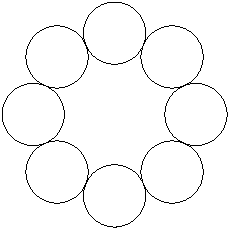
\includegraphics{circles.mps}}
  \end{center}
	\caption{Rotated circles}
  \label{fig:circles}
\end{figure}

The programming language constructs of \MP{} also deliver a graceful
mechanism for creating animations without having to manually create each
frame of the animation.  The primary advantage of \EPS{} is that it can
be scaled to any resolution without a loss in quality.  It can also be
easily converted to raster formats, e.g.\ Portable Network Graphics
(\PNG) and Joint Photographic Experts Group (\JPEG), et al., or other
vector formats including Portable Document Format (\PDF) and Scalable
Vector Graphics (\SVG), et al.

\begin{figure*}[tp]
  \centering
  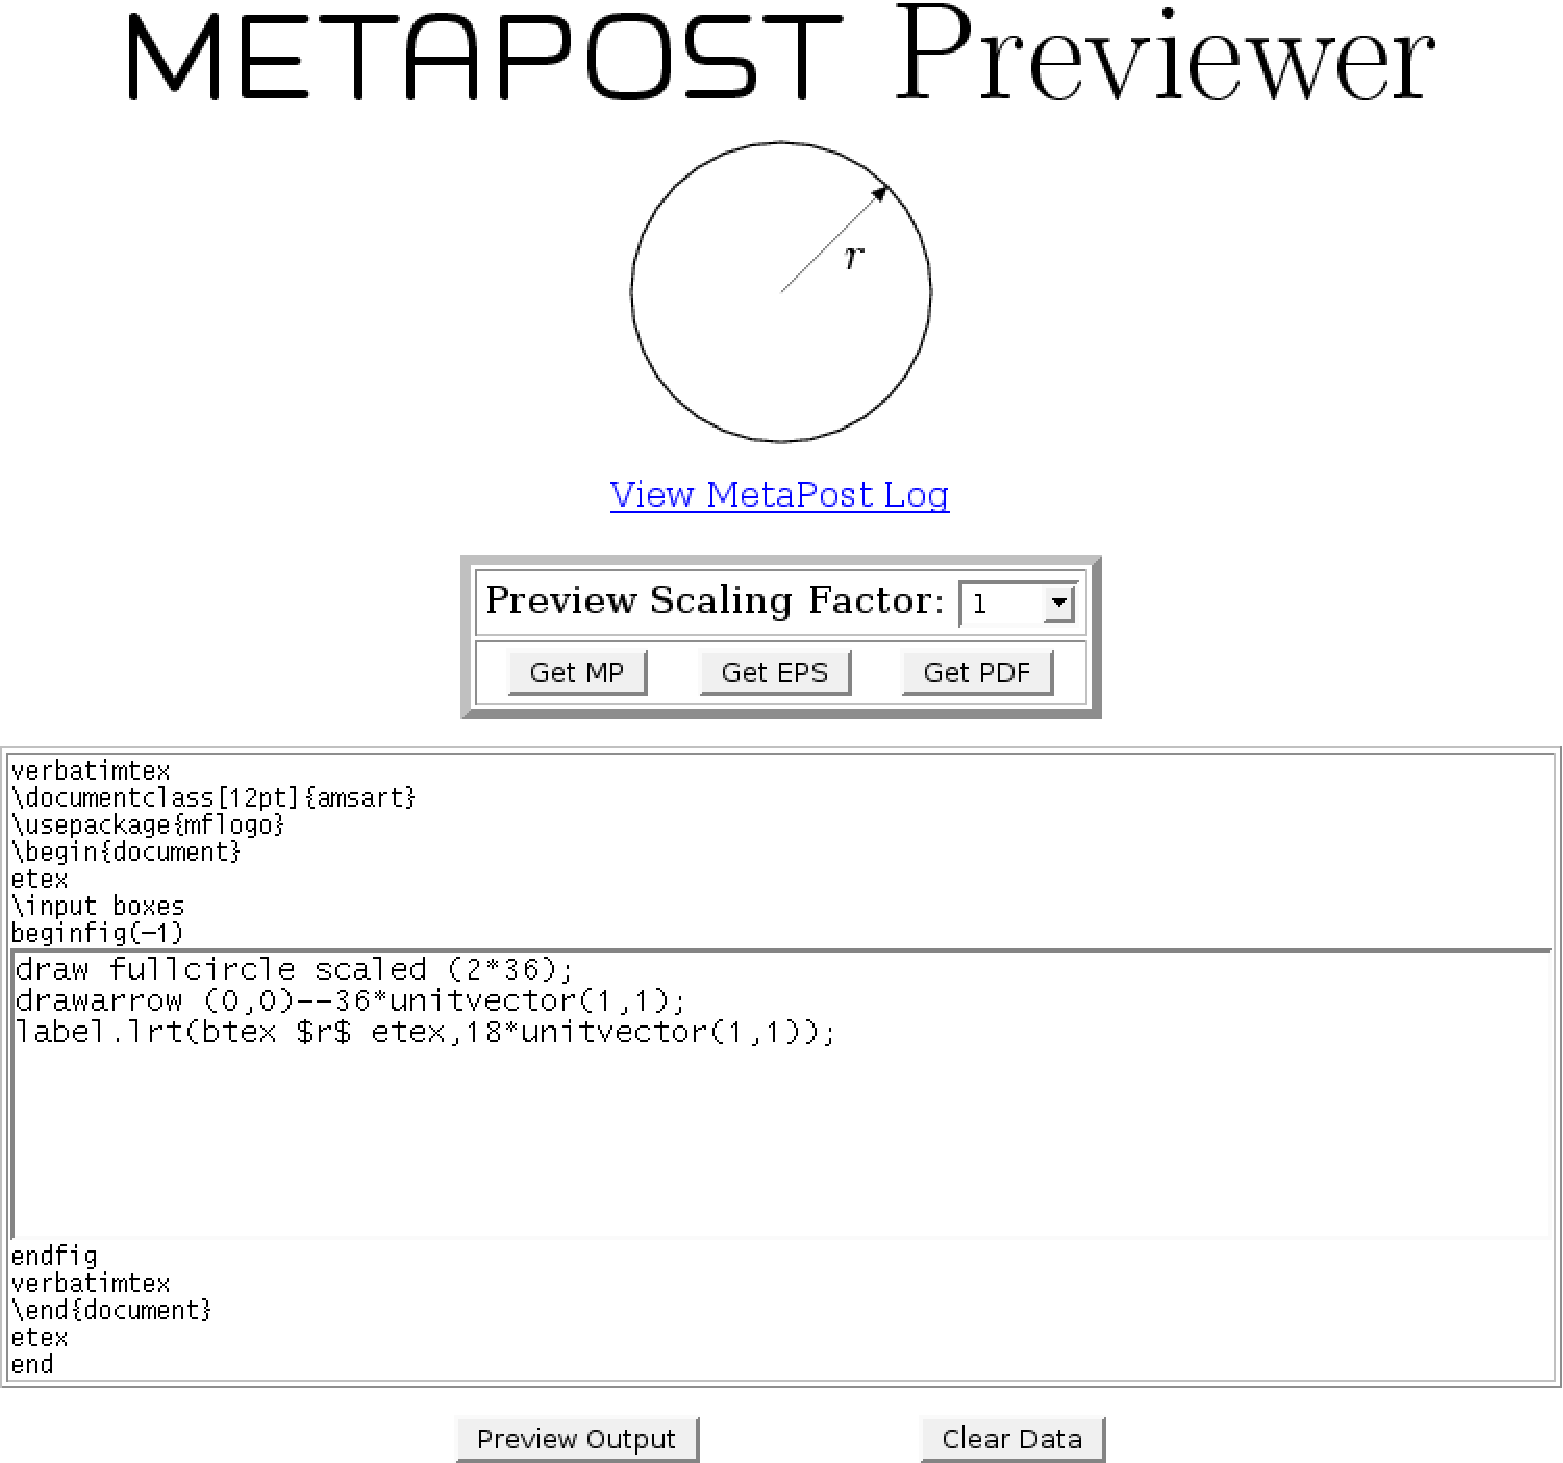
\includegraphics[width=\textwidth]{previewer}
  \caption{\MP{} Previewer}
  \label{fig:previewer}
\end{figure*}

\section{\MP{} compilation}
\label{sec:mpcompilation}

A typical \MP{} source file consists of one or more figures.
Compilation of the source file generates an \EPS{} graphic for each
figure.  These \EPS{} graphics are self-contained (i.e., the fonts used
in labels are embedded into the graphic) provided that
\lstinline{prologues:=3} is declared.

If \texttt{foo.mp} is a typical \MP{} source file, then its contents are
likely of the following form:

\begin{lstlisting}[xleftmargin=1.25\parindent]
prologues:=3;
outputtemplate:="%j-%c.mps";
beginfig(1);
   |\normalfont\textit{draw commands}|
endfig;
beginfig(2);
   |\normalfont\textit{draw commands}|
endfig;
|\dots|
beginfig(|\normalfont$n$|);
   |\normalfont\textit{draw commands}|
endfig;
end
\end{lstlisting}

Executing
\begin{flushleft}
  \hspace*{1.25\parindent}\texttt{mpostfoo.mp}
\end{flushleft}
yields the following output:

\begin{lstlisting}[xleftmargin=1.25\parindent]
This is MetaPost, Version |\normalfont$\langle$\textit{version}$\rangle$|
(foo.mp [1] [2] |\normalfont\ldots| [|\normalfont$n$|] )
|\normalfont$n$| output files written: foo-1.mps .. foo-|\normalfont$n$|.mps
Transcript written on foo.log.
\end{lstlisting}

For users who just want to ``get started'' using \MP{}, a \MP{}
previewer is available at \url{http://www.tlhiv.org/mppreview}.  This
previewer (illustrated in \autoref{fig:previewer}) is simply a graphical
interface to \MP{} itself.  It generates a single graphic with the
option to save the output in \EPS{}, \PDF{}, and \SVG{} formats.  Users
may also choose to save the source code and can view the compilation log
to assist in debugging.

\begin{section}{Data types}
  There are ten data types in \MP{}: \textit{numeric}, \textit{pair},
  \textit{path}, \textit{transform}, \textit{rgbcolor},
  \textit{cmykcolor}, \textit{string}, \textit{boolean},
  \textit{picture}, and \textit{pen}.  These data types allow users to
  store fragments of the graphics for later use.  We will briefly
  discuss each of these data types and elaborate on how they are used in
  a typical \MP{} program.
  \renewcommand{\labelitemi}{$\diamond$}
\begin{itemize}
	\item \textit{numeric}\Dash numbers
	\item \textit{pair}\Dash ordered pairs of numerics
	\item \textit{path}\Dash B\'{e}zier curves (and lines)
	\item \textit{picture}\Dash pictures
	\item \textit{transform}\Dash transformations such as shifts,\\rotations, and slants
	\item \textit{rgbcolor} or \textit{color}\Dash triplets with each component between $0$ and
    $1$ (red, green, and blue)
	\item \textit{cmykcolor}\Dash quadruplets with each component between $0$ and
    $1$ (cyan, magenta, yellow, and black)
	\item \textit{string}\Dash strings of characters
	\item \textit{boolean}\Dash ``true'' or ``false'' values
	\item \textit{pen}\Dash stroke properties
\end{itemize}

Virtually all programming languages provide a way of storing and
retrieving numerical values.  This is precisely the purpose of the
\textit{numeric} data type in \MP.  Since graphics drawn with \MP{} are
simply two dimensional pictures, it is clear that an ordered pair is
needed to identify each point in the picture.  The \textit{pair} data
type provides this functionality.  Each point in the plane consists of
an $x$ (i.e., abscissa) part and a $y$ (i.e., ordinate) part.  \MP{}
uses the standard syntax for defining points in the plane, e.g.,
\texttt{(}\textit{x}\texttt{,}\textit{y}\texttt{)} where both $x$ and
$y$ are numeric data typed variables.

In order to store paths between points, the \textit{path} data type is
used.  All paths in \MP{} are represented as cubic B\'{e}zier curves.
Cubic B\'{e}zier curves are simply parametric splines of the form
$(x(t),y(t))$ where both $x(t)$ and $y(t)$ are piecewise cubic
polynomials of a common parameter $t$.  Since B\'{e}zier curves are
splines, they pairwise interpolate the points.  Furthermore, cubic
B\'{e}zier curves are diverse enough to provide a ``smooth'' path
between all of the points for which it interpolates.  \MP{} provides
several methods for affecting the B\'{e}zier curve between a list of
points.  For example, piecewise linear paths (i.e., linear splines) can
be drawn between a list of points since all linear polynomials are also
cubic polynomials.  Furthermore, if a specific direction for the path is
desired at a given point, this constraint can be forced on the
B\'{e}zier curve.

The \textit{picture} data type is used to store an entire picture for
later use.  For example, in order to create animations, usually there
are objects that remain the same throughout each frame of the animation.
So that these objects do not have to be manually drawn for each frame, a
convenient method for redrawing them is to store them into a picture
variable for later use.

When constructing pairs, paths, or pictures in \MP{}, it is often
convenient to apply affine transformations to these objects.  As
mentioned above, Figure \ref{fig:circles} can be constructed by rotating
the same circle several times before drawing it.  \MP{} provides
built-in affine transformations as ``building blocks'' from which other
transformations can be constructed.  These include shifts, rotations,
horizontal and vertical scalings, and slantings.

For creating colored graphics, \MP{} provides two data types:
\textit{rgbcolor} and \textit{cmykcolor}.  These data types correspond
to the two supported color models \RGB{} and \CMYK.  While using the
\RGB{} color model, fractions of the primary colors
\textit{red}~\showcol{red}, \textit{green}~\showcol{green}, and
\textit{blue}~\showcol{blue} are ``additively mixed''.  Similarly, in
the \CMYK{} color model, the primary colors
\textit{cyan}~\showcol{cyan}, \textit{magenta}~\showcol{magenta},
\textit{yellow}~\showcol{yellow}, and \textit{black}~\showcol{black} are
``subtractively mixed.''  The former model is suitable for on-screen
viewing whereas the latter model is preferred in high-quality print.
Both color types are ordered tuples, $(c_1,c_2,c_3)$ and
$(c_1,c_2,c_3,c_4)$, with components~$c_i$ being \textit{numeric}s
between $0$ and $1$.  For example, in the \RGB{} color model,
\texttt{(1,0,0)} refers to red, whereas in the \CMYK{} color model
\texttt{(0,.6,1,0)} corresponds to an orange
tone~\showcol[cmyk]{0,.6,1,0}.  If a particular color is to be used
several times throughout a figure, it is natural to store this color
into a variable of type \textit{rgbcolor} or \textit{cmykcolor}.

The data type \textit{color} is a convenient synonym for
\textit{rgbcolor}.  Additionally, there are five built-in \RGB{} colors
in \MP{}: \texttt{black}, \texttt{white}, \texttt{red}, \texttt{green},
and \texttt{blue}.  So, in the example above \texttt{(1,0,0)} could
simply be replaced by \texttt{red} and \texttt{.4(red+blue)} refers to a
dark violet~\showcol[rgb]{.4,0,.4} in the \RGB{} color model.

The most common application of \textit{string} data types is reusing a
particular string that is typeset (or labeled).  The \textit{boolean}
data type is the same as in other programming languages and is primarily used in
conditional statements for testing.  Finally, the \textit{pen} data type
is used to affect the actual stroke paths.  The default unit of
measurement in \MP{} is $1\,\mathrm{bp}=1/72\mathrm{\ in}$, and the
default thickness of all stroked paths is $0.5\,\mathrm{bp}$.  An
example for using the \textit{pen} data type may include changing the
thickness of several stroked paths.  This new pen can be stored and then
referenced for drawing each of the paths.
\end{section}

\section{Common commands}
\label{sec:commoncmds}

The \MP{} manual \cite{hobby:user} lists 26 built-in commands along with
23 function-like macros for which pictures can be drawn and manipulated
using \MP.  We will not discuss each of these commands here; however, we
will focus on several of the most common commands and provide examples
of their usage.

\begin{subsection}{The \texttt{draw} command}
The most common command in \MP{} is the \texttt{draw} command.  This command is used to draw paths or pictures.  In order to draw a path from \texttt{z1:=(0,0)} to \texttt{z2:=(54,18)} to \texttt{z3:=(72,72)}, we should first decide how we want the path to look.  For example, if we want these points to simply be connected by line segments, then we use \begin{center}\verb|draw z1--z2--z3;|\end{center}  However, if we want a smooth path between these points, we use \begin{center}\verb|draw z1..z2..z3;|\end{center}  In order to specify the direction of the path at the points, we use the \texttt{dir} operator.  In Figure \ref{fig:draw1} we see that the smooth path is horizontal at \texttt{z1}, a 45\textdegree\ angle at \texttt{z2}, and vertical at \texttt{z3}.  These constraints on the B\'{e}zier curve are imposed by \begin{center}\verb|draw z1{right}..z2{dir 45}..{up}z3;|\end{center}
\begin{figure}[hptb]
	\begin{center}\textattachfile[color={0 0 0},mimetype={text/plain}]{draw.mp}{\includegraphics{draw-1.mps}}\end{center}
	\caption{\texttt{draw} examples}\label{fig:draw1}
\end{figure}
Notice that \verb|z2{dir 45}| forces the \textit{outgoing} direction at \texttt{z2} to be 45\textdegree.  This implies an \textit{incoming} direction at \texttt{z2} of 45\textdegree.  In order to require different incoming and outgoing directions, we would use \begin{center}\verb|draw z1{right}..{dir |$\theta_i$\verb|}z2{dir |$\theta_o$\verb|}..{up}z3;|\end{center} where $\theta_i$ and $\theta_o$ are the incoming and outgoing directions, respectively.
\end{subsection}

\begin{subsection}{The \texttt{fill} Command}
Another common command in \MP{} is the \texttt{fill} command.  This is used to fill closed paths (or cycles).  In order to construct a cycle, \texttt{cycle} may be appended to the path declaration.  For example,
\begin{lstlisting}[xleftmargin=7bp]
path p;
p:=z1{right}..z2{dir 45}..{up}z3--cycle;
fill p withcolor red;
draw p;
\end{lstlisting}
produces Figure \ref{fig:fill}.  Notice that \texttt{p} is essentially the same curved path as in Figure \ref{fig:draw1} with the additional piece that connects \texttt{z3} back to \texttt{z1} with a line segment using \texttt{-{}-cycle}.
\begin{figure}[t]
	\begin{center}\textattachfile[color={0 0 0},mimetype={text/plain}]{fill.mp}{
\includegraphics{fill}}\end{center}
	\caption{\texttt{fill} example}\label{fig:fill}
\end{figure}

Just as it is necessary to fill closed paths, it may also be necessary to \textit{unfill} closed paths.  For example, the annulus in Figure \ref{fig:annulus1} can be constructed by
\begin{lstlisting}[xleftmargin=38bp]
color bbblue;
bbblue:=(3/5,4/5,1);
path p,q;
p:=fullcircle scaled (2*54);
q:=fullcircle scaled (2*27);
fill p withcolor bbblue;
unfill q;
draw p;
draw q;
\end{lstlisting}
The \texttt{fullcircle} path is a built-in path that closely approximates a circle in \MP{} with diameter 1\,bp traversed counter-clockwise.  This path is not exactly a circle since it is parameterized by a B\'{e}zier curve and not by trigonometric functions; however, visually it is essentially indistinguishable from an exact circle.
\begin{figure}[t]
	\begin{center}\textattachfile[color={0 0 0},mimetype={text/plain}]{annulus_1.mp}{
\includegraphics{annulus_1}}\end{center}
	\caption{\texttt{unfill} example}\label{fig:annulus1}
\end{figure}
Notice that \texttt{p} is a \texttt{fullcircle} of radius 54\,bp (3/4\,in) and \texttt{q} is a \texttt{fullcircle} of radius 27\,bp (3/8\,in).  The annulus is constructed by filling \texttt{p} with the baby blue color \texttt{bbblue} and then unfilling \texttt{q}.  The \texttt{unfill} command above is equivalent to \begin{center}\verb|fill q withcolor background;|\end{center} where \texttt{background} is a built-in color which is \texttt{white} by default.

Often the \texttt{unfill} command appears to be the natural method for constructing figures like Figure \ref{fig:annulus1}.  However, the \texttt{fill} and \texttt{unfill} commands in Figure \ref{fig:annulus1} can be replaced by \begin{center}\verb|fill p--reverse q--cycle withcolor bbblue;|\end{center}
\begin{figure}[t]
	\begin{center}\textattachfile[color={0 0 0},mimetype={text/plain}]{annulus_2.mp}{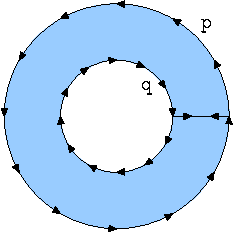
\includegraphics{annulus_2}}\end{center}
	\caption{Avoiding an \texttt{unfill}}\label{fig:annulus2}
\end{figure}
The path \verb|p--reverse q--cycle| travels around \texttt{p} in a counter-clockwise directions (since this is the direction that \texttt{p} traverses) followed by a line segment to connect to \texttt{q}.  It then traverses clockwise around \texttt{q} (using the \texttt{reverse} operator) and finally returns to the starting point along a line segment using \texttt{-{}-cycle}.  This path is illustrated in Figure~\ref{fig:annulus2}.  One reason for using this method to construct the annulus as opposed to the \texttt{unfill} command is to ensure \textit{proper transparency} when placing the figure in an external document with a non-white background.  If the former method is used and the annulus is placed on a non-white background, say magenta, then the result is Figure \ref{fig:annulus3}.
\begin{figure}[ht]
	\begin{center}\textattachfile[color={0 0 0},mimetype={text/plain}]{annulus_3.mp}{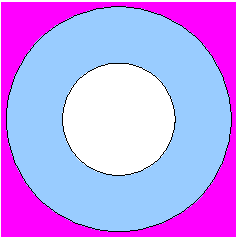
\includegraphics{annulus_3}}\end{center}
	\caption{Improper transparency using \texttt{unfill}}\label{fig:annulus3}
\end{figure}
It may be desired to have the interior of \texttt{q} be magenta instead of \texttt{white}.  This could be accomplished by redefining \texttt{background}; however, the latter method described above is a much simpler solution.
\end{subsection}

\subsection{Arrow commands}

When drawing simple graphs and other illustrations, the use of arrows is often essential.  There are two arrow commands in \MP{} for accommodating this need\Dash \texttt{drawarrow} and \texttt{drawdblarrow}.  Both of these commands require a path argument.  For example, \begin{center}\verb|drawarrow (0,0)--(72,72);|\end{center} draws an arrow beginning at \verb|(0,0)| and ending at \verb|(72,72)| along the line segment connecting these points.

The path argument of both \texttt{drawarrow} and \texttt{drawdblarrow} need not be line segmented paths\Dash they may be any \MP{} path.  The only difference between \texttt{drawarrow} and \texttt{drawdblarrow} is that \texttt{drawarrow} places an arrow head at the end of the path and \texttt{drawdblarrow} places an arrow head at the beginning and the end of the path.  As an example, to draw the curved path in Figure \ref{fig:draw1} with an arrow head at the end of the path (i.e., at \texttt{z3}), the following command can be used \begin{center}\verb|drawarrow z1{right}..z2{dir 45}..{up}z3;|\end{center} and is illustrated in Figure \ref{fig:draw2}.
\begin{figure}[ht]
	\begin{center}\textattachfile[color={0 0 0},mimetype={text/plain}]{draw.mp}{\includegraphics{draw-2.mps}}\end{center}
	\caption{Using \texttt{drawarrow} along a path}\label{fig:draw2}
\end{figure}

\subsection{The \texttt{label} command}

One of the nicest features of \MP{} is that it relies on \TeX{} (or
\LaTeX) to typeset labels within figures.  Almost all figures in
technical documents are accompanied by labels which help clarify the
situation for which the figure is assisting to illustrate.  Such labels
may include anything from simple typesetting as in
Figures~\ref{fig:draw1}, \ref{fig:annulus2}, and~\ref{fig:draw2} to
typesetting function declarations and even axes labeling.

The |label| command requires two arguments\Dash a string to typeset and
the point for which label is placed.  For example, the command

\begin{lstlisting}[style=MP]
label("A", (0,0));
\end{lstlisting}
will place the letter ``A'' at the coordinate |(0,0)| and the box around
this label is centered vertically and horizontally at this point.
Simple strings like \lstinline[style=text]{"A"} require no real
typesetting to ensure that they appear properly in the figure.  However,
many typeset strings in technical figures require the assistance of
\TeX{} to properly display them.

\begin{figure}
  \begin{withattachment}{parabola.mp}
    \centering
    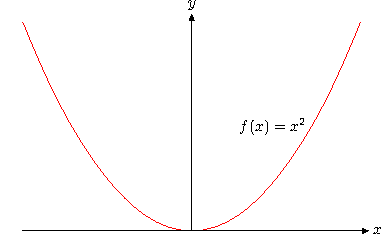
\includegraphics{parabola.mps}
  \end{withattachment}
  \caption{Labeling text}
  \label{fig:parabola}
\end{figure}

For example, \autoref{fig:parabola} is an example where typesetting is
preferred.  That is, the axes labels and the function declaration look
less than perfect if \TeX{} is not used.  For reasons such as this,
\MP{} provides a way to \textit{escape} to \TeX{} in order to assist in
typesetting the labels.  Therefore, instead of labeling the ``A'' as
above,

\begin{lstlisting}[style=MP]
label(btex A etex, (0,0));
\end{lstlisting}
provides a much nicer technique for typesetting the label.  The
|btex ... etex| block instructs \MP{} to process everything in between
|btex| and |etex| using \TeX.  Therefore, the function declaration in
\autoref{fig:parabola} is labeled using

\begin{lstlisting}[style=MP]
label(btex $f(x)=x^2$ etex, (a,b));
\end{lstlisting}
where $(a,b)$ is the point for which the label is to be centered.

Since many \MP{} users prefer to typeset their labels using \LaTeX{}
instead of plain \TeX, \MP{} provides a convenient method for
accommodating this, done in the preamble of the \MP{} source file.  The
following code ensures that the |btex ... etex| block escapes to
\LaTeX{} (instead of plain \TeX) for text processing.

\begin{lstlisting}[style=MP]
verbatimtex
%&latex
\documentclass{minimal}
\begin{document}
etex
beginfig(|$n$|);
|\quad$\langle\mbox{\normalfont\textit{draw commands}}\rangle$|
endfig;
end
\end{lstlisting}

Often times it is desirable to typeset labels with a justification that
are not necessarily centered.  For example, one may wish to place an
``A'' centered horizontally about |(0,0)|, but placed above
|(0,0)|. \MP{} provides eight suffixes to accommodate such needs.  The
suffixes |.lft|, |.rt|, |.bot|, and |.top| align the label on the left,
right, bottom, and top, respectively, of the designated point.  A hybrid
of these four justifications provide four additional ones, namely,
|.llft|, |.ulft|, |.lrt|, and |.urt| to align the label on the lower
left, upper left, lower right, and upper right, respectively, of the
designated point.  For example,

\begin{lstlisting}[style=MP]
label.top(btex A etex, (0,0));
\end{lstlisting}
places the ``A'' directly above |(0,0)|.  \autoref{fig:label}
demonstrates each of the suffixes and their corresponding placement of
the labels.

\begin{figure}
  \begin{withattachment}{label.mp}
    \hfill%
    \includegraphics{label-1.mps}%
    \hfill%
    \includegraphics{label-2.mps}%
    \hfill\mbox{}%
  \end{withattachment}
  \caption{Label suffixes}
  \label{fig:label}
\end{figure}


\section{Graphing functions}
\label{sec:graphing}

Among the most common types of figures for \TeX{} users are those which
are the graphs of functions of a single variable.  Hobby recognized this
and constructed a package to accomplish this task.  It is invoked by

\begin{lstlisting}[xleftmargin=80bp]
input graph;
\end{lstlisting}

\MP{} has the ability to construct data (i.e., ordered pairs) for
graphing simple functions.  However, for more complicated functions, the
data should probably be constructed using external programs such as
\acro{MATLAB} (or Octave), Maple, Mathematica, Gnuplot, et. al.

A typical data file, say \texttt{data.d}\attach{data.d}, to be used with
the \texttt{graph} package may have contents

\lstinputlisting[xleftmargin=77bp]{data.d}

This data represents the graph of $f(x)=\sqrt{x}$ for six equally spaced
points in $[0,1]$.  To graph this data, the size of the graph must first
be decided.  Choosing a width of $144\mathrm{\ bp}$ and a height of
$89\mathrm{\ bp}$, a minimally controlled plot (as in Figure
\ref{fig:data}) of this data can be generated by

\begin{lstlisting}[xleftmargin=38bp]
draw begingraph(144bp,89bp);
   gdraw "data.d";
endgraph;
\end{lstlisting}

The \texttt{graph} package provides many commands used to customize
generated graphs, and these commands are fully documented in the manual
\cite{hobby:graph} for the \texttt{graph} package.

\begin{figure}
  \centering
  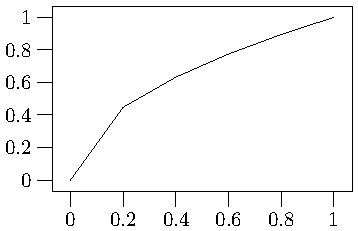
\includegraphics{data.mps}
  \caption{$f(x)=\sqrt{x}$ using the \texttt{graph} package}
  \label{fig:data}
  \attach{data.mp}
\end{figure}

\begin{section}{Including \MP{} figures in \LaTeX}
In order to include a \MP{} figure in \LaTeX{}, the \texttt{graphicx} package is suggested.  Below is an example of including a \MP{} figure (with name \texttt{foo-1.mps}) in a \LaTeX{} document.
\begin{lstlisting}[xleftmargin=17bp]
\documentclass{article}
\usepackage{graphicx}
\begin{document}
|\dots|
\includegraphics{foo-1.mps}
|\dots|
\end{document}
\end{lstlisting}
Having a \verb|.mps| file extension on the graphic allows the same graphic to be included in both \LaTeX{} and \PDF\LaTeX{} documents.  When using \PDF\LaTeX, the EPS graphic (with file extension \verb|.mps|) is converted to \PDF{} ``on the fly'' using Hans Hagen's \texttt{mptopdf}.  This conversion is necessary since \PDF\LaTeX{} performs no \PS{} processing.
\end{section}

\section{Conclusion}
\label{sec:conclusion}

\MP{} is an elegant programming language, and it produces beautiful
graphics.  The graphics are vectorial and thus can be scaled to any
resolution without degradation.  There are many advanced topics that are
not discussed in this article (e.g., loops, flow control, subpaths,
intersections, etc.), and the \MP{} manual~\cite{hobby:user} is an
excellent resource for these advanced topics.  However, the \MP{} manual
may seem daunting for beginners.  There are many websites containing
\MP{} examples, and several of these are referenced at
\url{http://www.tug.org/metapost}.  Finally, we mention that Knuth uses
nothing but \MP{} for his diagrams.

% \newpage
\bibliographystyle{plain}
\bibliography{mpguide}


\end{document}
